\documentclass[a4paper]{article}
\title{Notes for July 29}
\author{Johnicholas Hines}
\date{\today}
\renewcommand\today{July 23, 2021}


% Things that start with a % (percent sign) are ignored by LaTeX.  They are `comments' and are set off in blue on writeLaTeX.com.  They will never appear in the final output.

\usepackage{mathtools} % for align*
\usepackage{amsthm} % for environment proof

\usepackage{tikz}
\usetikzlibrary{cd} % for commutative diagrams

%\usepackage{graphicx}            % easy inclusion and manipulation of images
%\usepackage{microtype}           % just for fun: really hone in with the typography
%\usepackage{booktabs}            % nice looking tables that present the content first and foremost
%\usepackage{multicol}            % multiple columns in a local context
\usepackage[hidelinks]{hyperref} % clickable references in the output, but hide them visually

% These are called macros.  They aren't actually this simple, but you can think of it like a smart `find and replace' for most of your needs.
% Macros are case-sensitive.   See section 2.

% These two lines tell LaTeX that I want to
% 1) create a new piece of markup called `term' that takes one `thing' and puts single quotes around it
% 2) create a new piece of markup called `pkg' that takes one `thing' and sets it in a sans-serif font
% 3) redefine an existing piece of markup that doesn't take any `things' and just puts the text you see there.
%\newcommand\term[1]{`#1'}
%\newcommand\pkg[1]{\textsf{#1}}
%\newcommand\writeLaTeX{{\sffamily Overleaf}}
% The above macro (\writeLaTeX) is a good example of when macros come in handy.  This online service recently rebranded itself from 'writeLaTeX' to 'Overleaf'.  All references to the company have been replaced with this one change!  In all honesty this is not *unique* to TeX, but it is exceptionally *easy* in TeX.

% The next few macros use moderately advanced TeX.  They've been fine-tuned for appearance according to personal taste; you should never have to worry about this in your documents.  Ignore these macros except for the logical meanings: `control sequence' (formal term for a TeX macro) and `environment'.
\newcommand\embrace[1]{\texttt{\char`\{#1\char`\}}}
\newcommand\env[1]{\embrace{#1}}
\newcommand\cs[1]{\texttt{\string#1}}
\newcommand\csarg[2]{\cs{#1}\embrace{#2}}

\newtheorem{theorem}{Theorem}

\DeclareMathOperator{\B}{B}

\begin{document}
\maketitle

\begin{abstract}
TODO: write an abstract
\end{abstract}

%\tableofcontents

\section{The Eckmann-Hilton argument}

The Eckmann-Hilton argument, as far as I understand it, says that if something (such as a 2-dimensional homotopy group or a 2-dimensional category-like thing) is a monoid in two apparently different ways, but the apparently different operators are compatible with one another in a moderately nice way, then actually the two monoid operators are identical, and moreover the monoid operation is commutative.

\begin{theorem}
Suppose \( \star \) and \( \circ \) are two binary operators, with units, on the 
same set and further suppose that one distributes over the other: \( 
(a \star b) \circ (c \star d) = (a \circ c) \star (b \circ d) \). Then
\[
a \star  b = a \circ b = b \star a 
\]
\end{theorem}

\begin{proof}
  \begin{align*}
      a \star b = & (a \circ 1_\circ) \star (1_\circ \circ b) \\
      = & (a \star 1_\circ) \circ (1_\circ \star b) \\
      = & (a \circ b) \\
      = & (1 \star a) \circ (b \star 1) \\
      = & (1 \circ b) \star (a \star 1) \\
      = & b \star a
  \end{align*}
\end{proof}

We will now use \(\otimes\) for the operator; the distributive law now 
looks like \((a \otimes b) \otimes (c \otimes d) = (a \otimes c)
\otimes (b \otimes d)\).

\begin{theorem}
Suppose \( \star \) and \( \circ \) are two binary operators, with units, on the 
same set and further suppose that one distributes over the other:
\( (a \star b) \circ (c \star d) = (a \circ c) \star (b \circ d) \). 
Their units are identical.
\end{theorem}

\begin{proof}
  \begin{align*}
      1_\star = & 1_\star \otimes 1_\circ = 1_\circ
  \end{align*}
\end{proof}

Now we will use \(1\) to refer to the single identity.

\begin{theorem}
Suppose \( \star \) and \( \circ \) are two binary operators, with units, on the 
same set and further suppose that one distributes over the other:
\( (a \star b) \circ (c \star d) = (a \circ c) \star (b \circ d) \).
Then the operator is associative. 
\end{theorem}

\begin{proof}
\begin{align*}
(a \otimes b) \otimes c = & (a \otimes b) \otimes (1 \otimes c) \\
= & (a \otimes 1) \otimes (b \otimes c) \\
= & a \otimes (b \otimes c)
\end{align*}
\end{proof}


I did not learn the Eckmann--Hilton argument from the primary source; I 
tried to read the primary source
%\cite{eckmann1962group}
and bounced 
off. I learned it from Eugenia Cheng's video:  
\url{https://www.youtube.com/watch?v=Rjdo-RWQVIY} and wikipedia: 
\url{https://en.wikipedia.org/wiki/Eckmann\%E2\%80\%93Hilton_argument}

\section{Metamathematical reflections}

You can sometimes argue for a fact `the fibre product maps to the cartesian product, in categories that have a terminal object', where your argument seems to be mentioning and manipulating objects and morphisms `inside' the category in question. You can sometimes find a similar, corresponding, or equivalent argument that mentions and manipulates categories and functors `outside' the category in question.

Let's suppose that there's some formal proof system that mentions and manipulates objects and morphisms.
Let's suppose that there's some formal proof system that mentions and manipulates categories and functors.
If we can systematically translate (some) proofs from one vocabulary to the other, that would be an example of metamathematical reasoning - a proof by induction on the structure of mathematical proofs is metamathematics.
(Metamathematics is mathematics, of course.)

It's quite common for recognizably `the same' arguments to recur, in an apparently different context and/or vocabulary.
For example, the combinator \(B : (A \to B) \to (C \to A) \to C \to B\) can be viewed as a tautological statement: `A implies B implies that C implies A implies C implies B', or it can be viewed as a statement about morphisms `Morphisms from an object A to an object B induce maps on the collection of morphisms from C to A to the collection of morphisms from C to B', or it can be viewed as a statement about categories and functors `The category of functors from functors from A to B to functors from C to A to functors from C to B is inhabited, for generic categories A, B, C.'

Let's call these `In some as-yet-unformalized sense the same thing, but different in the context where it arises', a `metamathematical reflection'. The term `metamathematical reflection' is supposed to indicate a degree of understanding of the relationship a bit more detailed than a mysterious, as-yet-unexplained coincidence, but a bit less than either
\begin{enumerate}
    \item a clear theorem about a general case that has several clear specializations, or
    \item a clear formal proof with multiple familiar semantic models where it can be interpreted.
\end{enumerate} 

(I also believe, though I don't have a good example, that there's also
routine reflections which extend `inside' the objects of a category. If you are reasoning about `elements' or `points' that are imagined to be `inside' a an object of a category, then the argument probably has reflections `up' or `outside' the object, regarding several objects and several maps within one category.)

\subsection{A monoidal category}

(This text is taken from Wikipedia) 

A monoidal category is a category \(\mathbf{C} \) equipped with a monoidal structure. A monoidal structure consists of:

\begin{itemize}
    \item a functor \(\otimes \colon \mathbf {C} \times \mathbf {C} \to \mathbf {C}\) called the tensor product or monoidal product,
    \item an object \( I \) called the unit object or identity object, and
    \item a natural (in each of three arguments \(A, B, C\) isomorphism \(\alpha\), called associator, with components
    \( \mathop{\alpha} A B C \colon A\otimes (B\otimes C) \to (A\otimes B)\otimes C\),
    \item two natural isomorphisms \(\lambda\)  and \(\rho\), respectively called left and right unitor, with components \( \mathop{\lambda} A \colon I\otimes A \to A\) and \(\mathop{\rho} A \colon A\otimes I \to A \)
\end{itemize}
The coherence conditions for these natural transformations are:
\begin{itemize}
    \item for all \(A, B, C\) and \(D\) in \(\mathbf {C}\), the pentagon diagram commutes:

% https://tikzcd.yichuanshen.de/
\begin{tikzcd}
& A \otimes (B \otimes (C \otimes D)) \arrow[ldd, "\operatorname{\alpha} A B (C \otimes D)" description] \arrow[rd, "(\operatorname{id} A) \otimes (\operatorname{\alpha} B C D)" description] & \\
& & A \otimes ((B \otimes C) \otimes D) \arrow[dd, "\operatorname{\alpha} A (B \otimes C) D" description] \\
(A \otimes B) \otimes (C \otimes D) \arrow[rdd, "\operatorname{\alpha} (A \otimes B) C D" description] & & \\
& & (A \otimes (B \otimes C)) \otimes D \arrow[ld, "(\operatorname{\alpha} A B C) \otimes (\operatorname{id} D)" description] \\
& ((A \otimes B) \otimes C) \otimes D &                   
\end{tikzcd}

    \item for all \(A\) and \(B\) in \(\mathbf{C}\), the triangle diagram commutes:

% https://tikzcd.yichuanshen.de/
\begin{tikzcd}
A \otimes (I \otimes B) \arrow[rr, "\mathop{\alpha} A I B" description] \arrow[rd, "(\mathop{id} A) \otimes (\mathop{\lambda} B)" description] & & (A \otimes I) \otimes B \arrow[ld, "(\mathop{\rho} A) \otimes (\mathop{id} B)" description] \\
& A \otimes B &                                                                                            
\end{tikzcd}
    
\end{itemize}

Aside: This definition is not obviously the correct categorification of the the concept of a monoid. I think the intent is something like `every equation that is true in a free monoid on the objects, with \(\otimes\) as binary operator and \(I\) as unit, has a corresponding isomorphism, and furthermore any two proofs, that a particular equation that is true in a free monoid on the objects, has a corresponding natural transformation'. 

Why did Mac Lane phrase it this way (where showing that this definition captures that intent is a theorem to be proved: Mac Lane's coherence theorem), rather than the other way (where showing that a monoidal category can be presented by a pentagon law plus a triangle law would be the theorem to be proved)? Maybe it was an accident / no meaning. Maybe it was a fashion in mathematics. Maybe it has something to do with infinities? I feel comfortable thinking about finite and countable things, and handwaving off bigger infinities, saying something like `if you care about bigger infinities, I am sure there's a generalization of the theorems regarding finite and countable things that would be relevant there' (Downward Lowenheim-Skolem:
\cite{lowenheim1915moglichkeiten, 
%skolem1919untersuchungen,
%skolem1922einige,
burris2001downward}) - but Mac Lane might not be that sort of mathematician? 

The pentagon is two closely related things, on the one hand, it is the local confluence of directed rewriting that (combined with well-ordering) yields global confluence and therefore a decision procedure, and an associahedron.

Knuth-Bendix completion is an algorithm that can turn a set of equational identities into a decision procedure, by first orienting the equations, and then finding `critical pairs', expressions that can be rewritten in more than one way. If all of the critical pairs can be replaced with a rewrite rule `completing' the critical pair, and those rewrite rules do not introduce further critical pairs, then Knuth-Bendix completion terminates with a confluent rewrite system. Running  There is a law of associativity, \( a ( b c ) = (a b) c \). If you choose to orient that law to the right, then you have a rewrite rule that reassociates things `to the left'. \( a ( b c ) \to (a b) c\) but you don't have a confluent rewrite system. Running Knuth-Bendix on the rewrite system consisting of the one rewrite rule, you will find there is a critical pair, an expression that can be rewritten in more than one way, the starting point of the pentagon. Completing the pentagon means adding a rewrite rule from the starting point to the ending point of the pentagon. With that rule, there are no more critical pairs, and so Knuth-Bendix returns with a confluent rewriting system. 

This leads to some natural questions:
\begin{enumerate}
    \item If you have an equational theory (such as the theory of rigs? According to \url{https://ncatlab.org/nlab/show/rig+category}, coherence for rig categories was worked out in (Laplaza 1972) and (Kelly 1974)?), by running Knuth-Bendix on it, you can find out what the analogs of the pentagon and the triangle laws would be, and so what the Mac Lane style categorification of that equational theory would be. See \cite{beke2011categorification}.
    \item There's a quality of rewrite rules, that typically mathematicians use patterns that match anywhere in an expression, but programmers for efficiency routinely use patterns that can only match at the root, and add `bureaucratic' or `administrative' rules that `walk' the root (with `chroot'-like rotations) through the whole term to be processed, explicitly. What would the categorification of this idea be? 
    \item If Buchberger's algorithm is an extension or variant of Knuth-Bendix, then you might wonder - what category-theoretic concepts do its outputs correspond to?
    \item If resolution is an extension or variant of Knuth-Bendix, then what category-theoretic concepts do its outputs correspond to?

\end{enumerate}


\section{A monoid object within a monoidal category}

A \emph{monoid object} in
\(\mathcal{C}\) is an object \(\mathbf{M}\) in \(\mathcal{C}\) together with
morphisms
\[ e \colon \mathbf{1} \to \mathbf{M} \quad\text{and}\quad  \mu \colon \mathbf{M} \otimes \mathbf{M} \to \mathbf{M} \]
such that the following two diagrams commute:

% https://tikzcd.yichuanshen.de/
\begin{tikzcd}
\mathbf{1} \otimes \mathbf{M} \arrow[rrdd, "\mathop{pr} 2" description] \arrow[rr, "\mathop{e} \otimes (\mathop{id} \mathbf{M})" description] &  & \mathbf{M} \otimes \mathbf{M} \arrow[dd, "\mu" description] &  & \mathbf{M} \otimes \mathbf{1} \arrow[ll, "(\mathop{id} \mathbf{M}) \otimes \mathop{e}" description] \arrow[lldd, "\mathop{pr} 1" description] \\
 &  &  &  &  \\
&  & \mathbf{M} &  &                                                                                                                                              
\end{tikzcd}

\quad\text{and}\quad

% https://tikzcd.yichuanshen.de/#N4Igdg9gJgpgziAXAbVABwnAlgFyxMJZABgBpiBdUkANwEMAbAVxiRAB12BbOnACwBGAM2ABZAL4ACThDxd407r0EiJi2VnlxFPfsLFSQ40uky58hFACZyVWoxZtOulQfVyFz5folGTIDGw8AiIbKzt6ZlZEDiU9VXE-UyCLIjJw6kjHGK94txkPbVzXX3E7GCgAc3giUCEAJwguJDIQHAgkAGZqBjoBGAYABTNgyxAsMGxYEEyHaJAACiwoHW8EgEp3TU84ksTjOsbmxG62jsQbEF7+oZHUmImp1lmop24mJJAGppbqdqQAIw9PoDYYpEIPSbLZ72V45d5bLSSJYrYo+cTrT7fY5As5IS7XUF3CHjKHTF7ZWJcD5lcRAA
\begin{tikzcd}
\mathbf{M} \otimes \mathbf{M} \otimes \mathbf{M}  \arrow[dd, "(id \mathbf{M}) \otimes \mathbf{M}" description] \arrow[rr, "\mu \otimes (id \mathbf{M})" description] &  & \mathbf{M} \otimes \mathbf{M} \arrow[dd, "\mu" description] \\
&  & \\
\mathbf{M} \otimes \mathbf{M} \arrow[rr, "\mu" description] &  & \mathbf{M}                                                 
\end{tikzcd}

Okay, we want to prove that the monoid object induces a monoid structure to the set of maps from a generic object into the monoid object.

ENDORSE: The combinator \(B\) lifts the \(e\) morphism to a map from morphisms into \(\mathbf{1}\) to morphisms into the monoid object. There is a unique map into the terminal object. So \(B e (X \to 1) : X \to M\) is a particular element of the set of morphisms from \(X \to M\). \footnote{Recall we are using Haskell-like syntax for function application, \(f x\) means `the result of applying the function \(f\) to \(x\)', and also we are using types as names of values, if there is only one relevant value of that type.} 

TRUE BUT DEAD END? Any two morphisms \(f: X \to M, g: X \to M\) corresponds
to a single morphism \(f \times g: X \times X \to M \times M\) in the product category.
That morphism is mapped by the \(\otimes\) functor to an arrow \( (\otimes) (f \times g) : X \otimes X \to M \otimes M \).

OBSTACLE: I don't see a way to get from \(X\) to \(X \otimes X\).

TRUE BUT DEAD END? The combinator \(B'\) is characterized by taking \(\mathop{B'} x y z \mapsto y (x z)\).
It can be given a type (which per usual is a tautology if \(\to\) is interpreted as implication):
\((A \to B) \to (B \to C) \to A \to C\). It sortof corresponds to the semicolon `followed by' or `flipped function composition' operator. If we apply \(\mathop{B'}\) to the monoid object map \(\mu\) we get \(\mathop{B'} \mu : (M \to X) \to M \otimes M \to X\). Not sure how that's helpful.

TRUE BUT DEAD END? The combinator \(B\) is characterized by \(\mathop{B} x y z \mapsto x (y z)\). 
It can be given a type: \((B \to C) \to (A \to B) \to A \to C\). It sortof corresponds to the \(\circ\) `function composition' operator. \(\mathop{B} \mu : (X \to M \otimes M) \to X \to M\)

TRUE BUT DEAD END? The combinator \(C\) is defined as \(\mathop{C} x y z \mapsto x z y\).
It can be given a type \((A \to B \to C) \to B \to A \to C\). It's some sort of curried commutativity principle. In order to use it, I need a something that is a map that goes into a function type.

TRUE BUT DEAD END? There's a principle that a map out of a product \(X \times Y \to Z\) is equivalent to a map into a function type \(X \to Y \to Z\). If we call that transformation \(\mathop{Curry}\),
then we could say that \( \mathop{Curry} (\otimes) : X \to Y \to X \otimes Y \). That's a map into an arrow type, but it wouldn't do us any good to apply \(C\) to it.

\(S\) is a combinator that might work. \( S : (A \to B \to C) \to (A \to B) \to A \to C\). 
\(S (\mathop{Curry} (\otimes)) : (X \to Y) \to X \to X \otimes Y\). Okay, that looks promising. 

Here's a sketch of a sketch of how to define a binary operator on morphisms \(f : X \to M, g : X \to M\):
\begin{itemize}
    \item \(S (\mathop{Curry} (\otimes)) \mathop{id} : X \to X \otimes X\).
    \item \( \mathop{B'} (S (\mathop{Curry} (\otimes)) \mathop{id}) (f \otimes g) : X \to M \otimes M\).
    \item \( \mathop{B'} (\mathop{B'} (S (\mathop{Curry} (\otimes)) \mathop{id}) (f \otimes g)) \mu : X \to M \).
\end{itemize}

TODO: use the monoid object laws to show that this binary operator is associative and respects the proposed identity element.

\section{DRY: Don't Repeat Yourself}

The skein tree is a technique for calculating knot invariants;
this illustration was drawn by Louis Kauffman, who invented the Kauffman polynomial, a knot invariant:

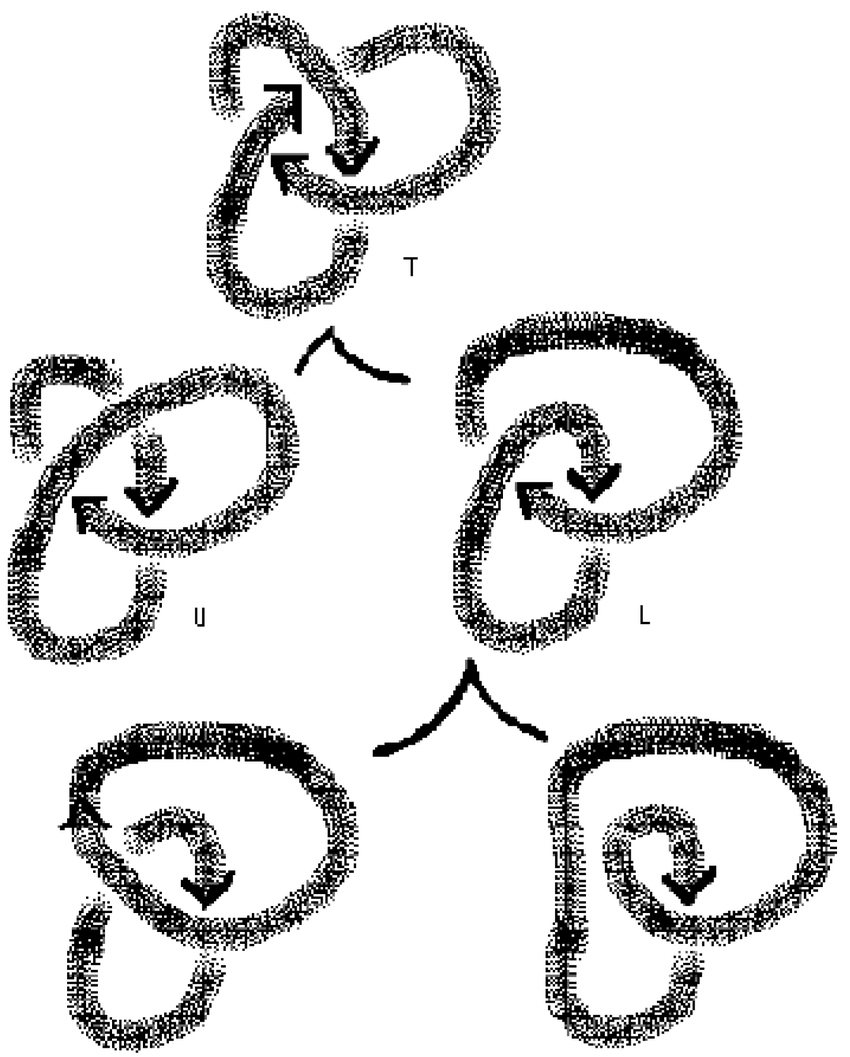
\includegraphics[scale=0.25]{images/The-Trefoil-Skein-Tree}

The illustration of the skein tree consists of multiple entire knots, which are connected together in a tree, where adjacent knots are related by being almost entirely duplicates, with a small exception at one crossing.

An equational proof, such as the Eckman-Hilton ones earlier, is not normally considered to be a diagram, but if you replace each of the expressions by its parse tree,
it is clear that the parse trees are related to one another in a chain, where they are almost entirely duplicated, with only a small exception (called the redex in term rewriting).

A Gentzen sequent proof \footnote{See for example \url{https://en.wikipedia.org/wiki/Sequent_calculus}, it's too disgusting to illustrate here} is not normally considered to be a diagram, but if you replace each of the sequents by its parse tree, the sequent proof forms a tree, where the parse trees of adjacent sequents are related to one another by being almost entirely duplicates, with only a small exception.

There's a slogan in programming: `Don't Repeat Yourself' - that suggests that `factoring out' this duplication would be a good thing to do.
That is, if you can turn aside from whatever project you
are working on to clear away a tangle of duplication (whether
you consider it `notation' or not), you can often see further,
and clearer, than if you kept plugging away in the usual way.



\bibliographystyle{amsplain}
\bibliography{refs}


\end{document}

\section{Some \LaTeX\ Examples}
\label{sec:examples}

%Now that you know the idea behind \LaTeX, let's get into some concrete examples.  If you haven't read the introduction (\autoref{sec:what-is}), I strongly urge you to; things from here on out will make more sense.  I encourage you to read along with the source; if you have been you already know how to
%  emphasize text with \cs\emph,
%  start a bulleted list with \env{itemize},
%  start a section with \cs\section,
%  give a footnote with \cs\footnote,
%  and use a cross-reference using \cs\label and \cs\autoref.\footnote{%
%    Actually, this command is given by the \pkg{hyperref} package.
%    The standard command to use is \cs\ref,
%      but \cs\autoref will insert the appropriate label in front
%      (like `section') when \pkg{hyperref} knows it.
%    Of course, you can teach the package new things.}
%You also know that \LaTeX\ doesn't really pay attention to
%  inconsistent        inter-word    spacing   or
%  random
%     line
%    breaks.  The only    real `rule':
%           if it encounters a \emph{blank} line---whitespace only---%
%           it starts     a new          paragraph.
           
% You can also `skip' spaces using the comment character.
% If you take the following, for example:
% 
%     Lorem ipsum doler---
%       sit amet.
% 
% You will see that there is an unwanted space after the dash.
% If we had a comment character to `comment out' the rest of the line:
% 
%     Lorem ipsum doler---%
%       sit amet.
% 
% This yields the desired result.

% Note also that it is generally poor practice to have excessively long lines -- it even makes your content harder for you to read while you're writing it -- so I make sure that my view of the content never makes the lines very long.  I will squeeze the window to be thinner (soft-wrapping the content) or tell my text editor to hard-wrap it into shorter lines to make sure I can easily read my content.  (Shorter lines also come in handy if you choose to use version control -- an advanced topic for another day.)

%\subsection{How to Organize Your Document}

%As you've already seen, \LaTeX\ comes with at least one command to organize your document: %\cs\section.  There are, in fact, many others:
%\begin{multicols}{3}
%\begin{enumerate}
%\item \cs\part
%\item \cs\chapter
%\item \cs\section
%\item \cs\subsection
%\item \cs\subsubsection
%\item \cs\paragraph
%\item \cs\subparagraph
%\end{enumerate}
%\end{multicols}
%Actually, the availability of these commands\footnote{Or \term{control sequences} as they are more properly called.} depends on the \term{document class} you use.  For example, \csarg\documentclass{article} doesn't define \cs\part or \cs\chapter, but \csarg\documentclass{book} does.

\subsection{How to Make Lists}
% Very slightly adapted from the stock text by writeLaTeX.com

You can make lists with automatic numbering using \env{enumerate}\dots
\begin{enumerate}
\item Like this,
\item and like this.
\end{enumerate}
\dots or bullet points using \env{itemize}\dots
\begin{itemize}
\item Like this,
\item and like this.
\end{itemize}
\dots or with words and descriptions using \env{description}\dots
\begin{description}
\item[Word] Definition
\item[Concept] Explanation
\item[Idea] Text
\end{description}

\subsection{How to Include Figures}
% adapted from the stock text by writeLaTeX.com

See the code for \autoref{fig:frog} in this section for an example.
\begin{enumerate}
\item Upload the image file (JPEG, PNG or PDF) from your computer to \writeLaTeX\ using the upload link the project menu.
\item Use the \cs\includegraphics command to include it in your document.
\item Use the \env{figure} environment and the \cs\caption command to add a number and a caption to your figure.
\end{enumerate}

\begin{figure}
\centering
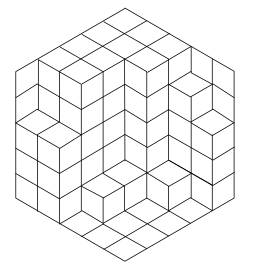
\includegraphics[width=0.3\textwidth]{images/hexagon}
\caption{This hexagon was uploaded to \writeLaTeX\ via the project menu.}
\label{fig:frog}
\end{figure}

\subsection{How to Make Tables}

Use the \env{table} and \env{tabular} commands for basic tables---see \autoref{tab:widgets} on page~\pageref{tab:widgets}, for example.  \cs\toprule, \cs\midrule, and \cs\bottomrule are all provided by \pkg{booktabs}.  The standard command to use is \cs\hline, but see the \pkg{booktabs} documentation\footnote{\url{http://texdoc.net/texmf-dist/doc/latex/booktabs/booktabs.pdf}} for some nice reading on why the tables it suggests are better.
% the \url command is provided by the `hyperref' package.

\begin{table}
\centering
\begin{tabular}{lr}
\toprule
Item & Quantity \\
\midrule
Widgets & 42 \\
Gadgets & 13 \\
\bottomrule
\end{tabular}
\caption{An example table.}
\label{tab:widgets}
\end{table}

\subsection{How to Write Mathematics}
% adapted from stock example for correctness and best practices

\LaTeX\ is great at typesetting mathematics.  Let $X_1, X_2, \ldots, X_n$ be a sequence of independent and identically distributed random variables with $\text{E}[X_i] = \mu$ and $\text{Var}[X_i] = \sigma^2 < \infty$, and let
\[S_n = \frac{X_1 + X_2 + \cdots + X_n}{n}
      = \frac{1}{n}\sum_{i}^{n} X_i\]
denote their mean.  Then as $n$ approaches infinity, the random variables $\sqrt{n}(S_n - \mu)$ converge in distribution to a normal $\mathcal{N}(0, \sigma^2)$.

% Back to totally me
I have no idea what \emph{any} of that means, so see \autoref{eq:simple}.
If you want to be concise about it, you can also use \cs\eqref: see~\eqref{eq:simple}.
\begin{thm}
  If this, then that.
\end{thm}
\begin{proof}
  Since we know that
  \begin{equation}
    \text{this} \implies \text{that},
    \label{eq:simple}
  \end{equation}
  the result directly follows.
\end{proof}
There is a lot more to mathematics typesetting, but that's beyond the scope of this article.  There may be another that looks at this in-depth.

\section{Getting Help}

\LaTeX\ comes with very thorough documentation.  For online use, simply Google-search \texttt{texdoc (package)} to look up the official documentation for \pkg{package}.  This mirrors the command-line tool, \texttt{texdoc}, which is used in the same way.  For everything else, usually a simple search for \texttt{LaTeX (thing)} for information on \cs\thing or \env{thing}.  For everything else, including specific help, there's the \TeX~StackExchange.\footnote{\url{http://tex.stackexchange.com}}

\section{Next Steps}

\subsection{Getting \LaTeX}

\writeLaTeX\ is a useful resource and I encourage you to use it to the fullest.  However, \LaTeX\ is a program that can run on \emph{your} computer just as easily as it can run online.  It is absolutely free.
My recommendations are as follows:
\begin{description}
\item[Windows] \TeX~Live\footnote{\url{http://www.tug.org/texlive/windows.html}} (but MiK\TeX\footnote{\url{http://www.miktex.org}} is another popular option).
\item[Mac] Mac\TeX\footnote{\url{http://www.tug.org/mactex}} is by \emph{far} the best.  I highly recommend it.
\item[Linuxes] \TeX~Live\footnote{\url{http://www.tug.org/texlive}} is your \emph{only} option, and I actually recommend against using your distribution's package manager to install it and encourage you to use install script provided upstream.  The versions are almost always several years behind, and \LaTeX\ package development is very active.  If you absolutely must use the package manager, install \texttt{texlive-full} or similar---trust me when I say that it makes life \emph{much} easier.
\end{description}

To make links easier to work with, download the PDF using the appropriate button above on the top bar.  This is what \LaTeX\ actually produced for \writeLaTeX; it is fully clickable and otherwise interactive.  (It also just looks \emph{nicer} somehow\dots)

\subsection{Choosing an Editor}

Your experience with \LaTeX\ will largely be impacted by your choice of editor.  For learning on any platform, TUG's own \TeX works is a good starting point.  When you find you're repeating yourself a lot, I recommend moving onto \TeX maker (also cross-platform).  If you are comfortable using it---I won't lie and say it's immediately intuitive for a beginner---the venerable Emacs editor has an excellent mode called \textsc{Auc\TeX}.  It is \emph{extremely} good.  \TeX maker and Emacs will see you through from then on, and both are absolutely free.

\vfill

\begin{center}
Happy \TeX ing!
\end{center}

\vfill
